\section{Approximate Abstraction on Example Domains}

Here we discuss the results shown in states blah blah \dnote{Description of this section}.


\begin{itemize}
\item For $\epsilon > 0$, there are extremely useful abstractions to be made. Want to emphasize that with approximate knowledge of X, can still abstract effectively (point out Minefield + NChain both retain a very good policy from abstract MDP). This hits the learnable point.
\item Explain goal based/Taxi (regenerate plot for different scale of epsilon)
\item Possibly talk about stochasticity (low priority)
\item Explain Random behavior, smooth interpolation, mention randomness, etc.
\item Describe plots a bit (what is the y-axis?)
\end{itemize}

% Figure: Epsilon vs. #States for all three sample domains.
\begin{figure}
\centering
\subfigure[NChain]{
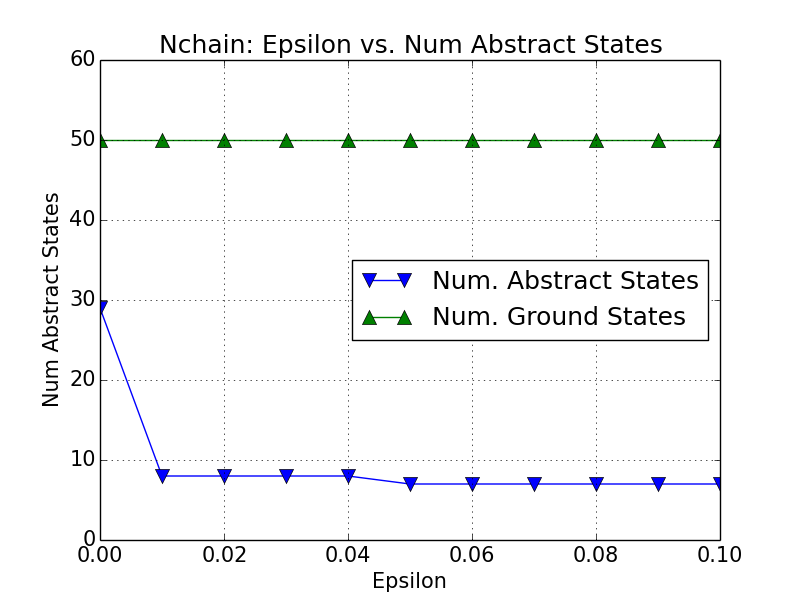
\includegraphics[width=0.48\columnwidth]{figures/nchain_epsilon_vs_num_abstract_states.png}}
\subfigure[Taxi]{
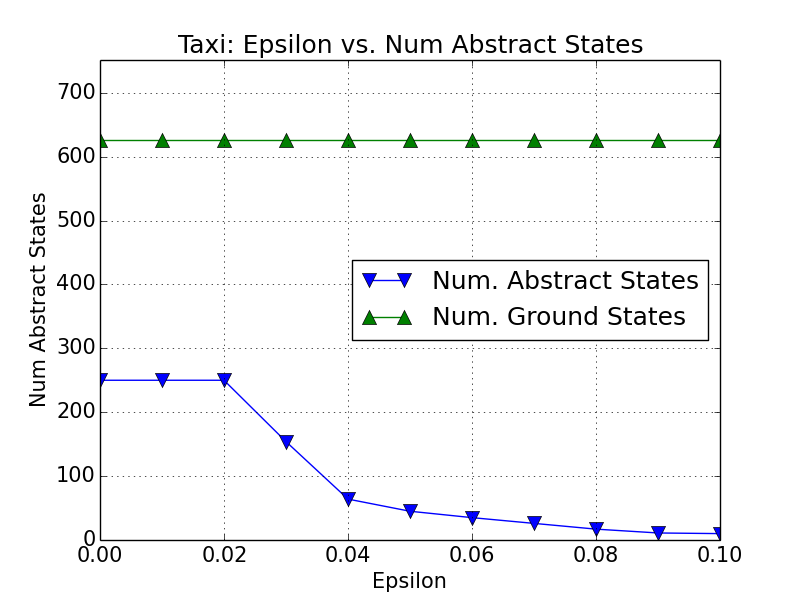
\includegraphics[width=0.48\columnwidth]{figures/taxi_epsilon_vs_num_abstract_states.png}}
\subfigure[Minefield]{
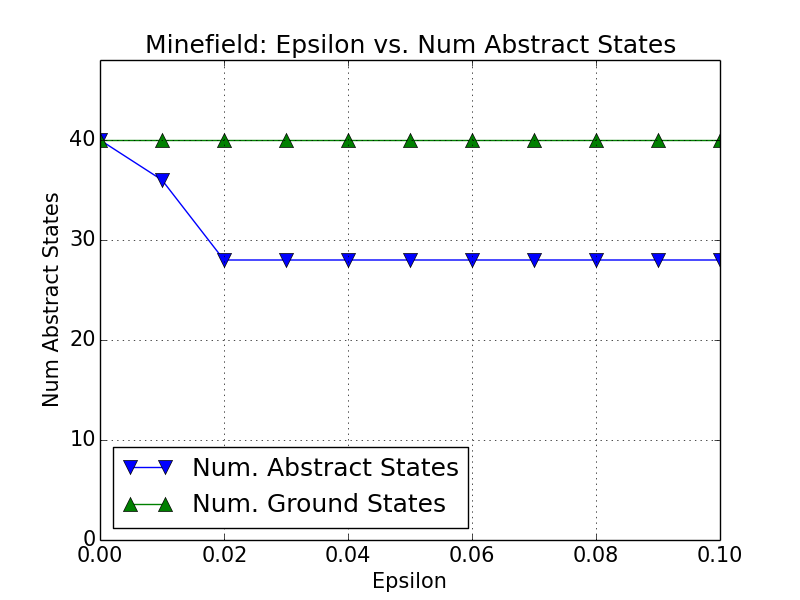
\includegraphics[width=0.48\columnwidth]{figures/minefield_epsilon_vs_num_abstract_states.png}}
\subfigure[Random]{
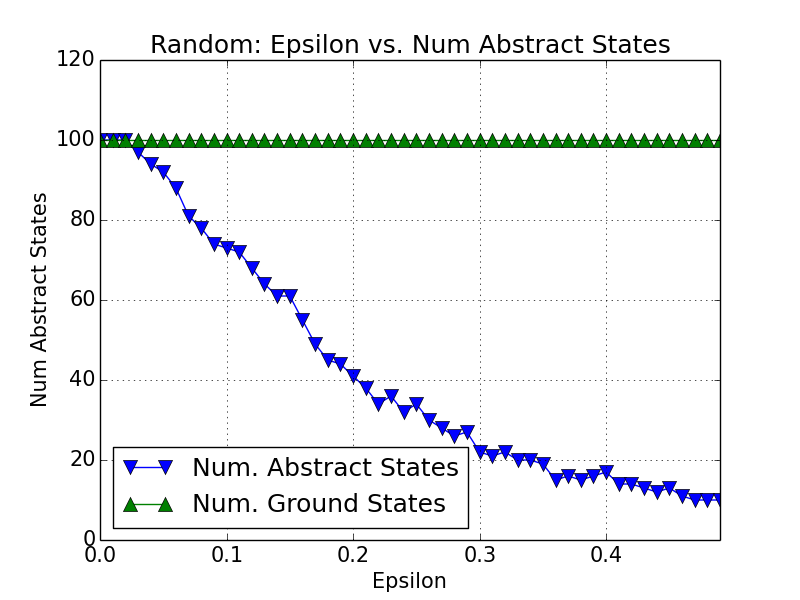
\includegraphics[width=0.48\columnwidth]{figures/random_epsilon_vs_num_abstract_states.png}}
\label{fig:eps-states}
\caption{$\epsilon$ vs. Num States}
\end{figure} 

% Figure: Epsilon vs. Error in Abstract Value Function
\begin{figure}
\subfigure[NChain]{
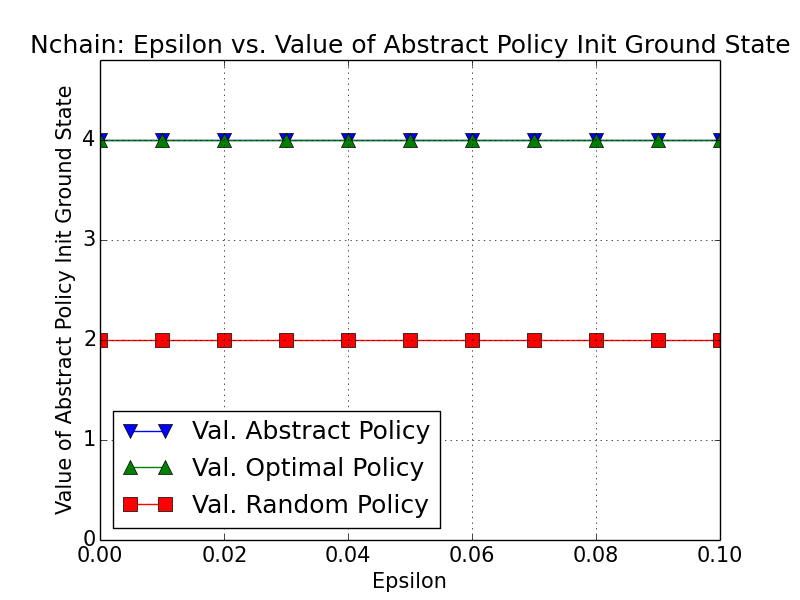
\includegraphics[width=0.48\columnwidth]{figures/nchain_epsilon_vs_value_of_abstract_policy_init_ground_state.png}}
\subfigure[Taxi]{
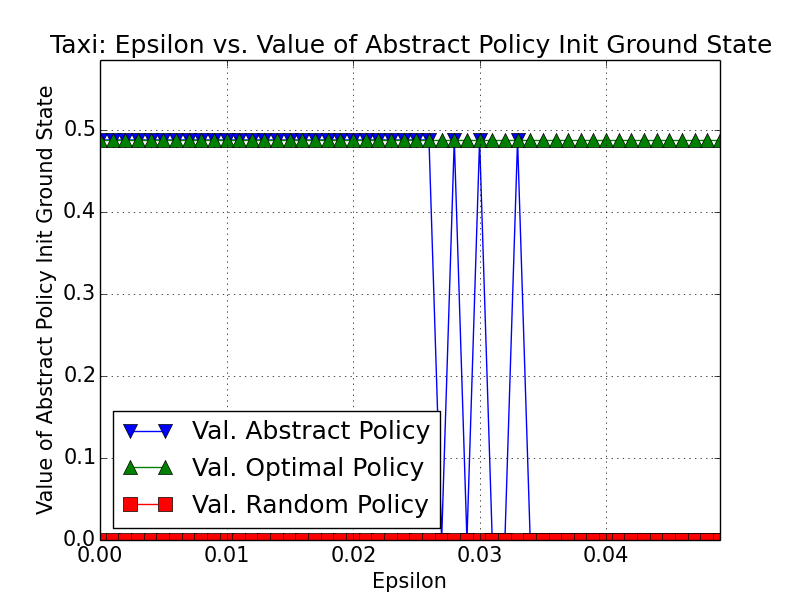
\includegraphics[width=0.48\columnwidth]{figures/taxi_epsilon_vs_value_of_abstract_policy_init_ground_state.png}}
\subfigure[Minefield]{
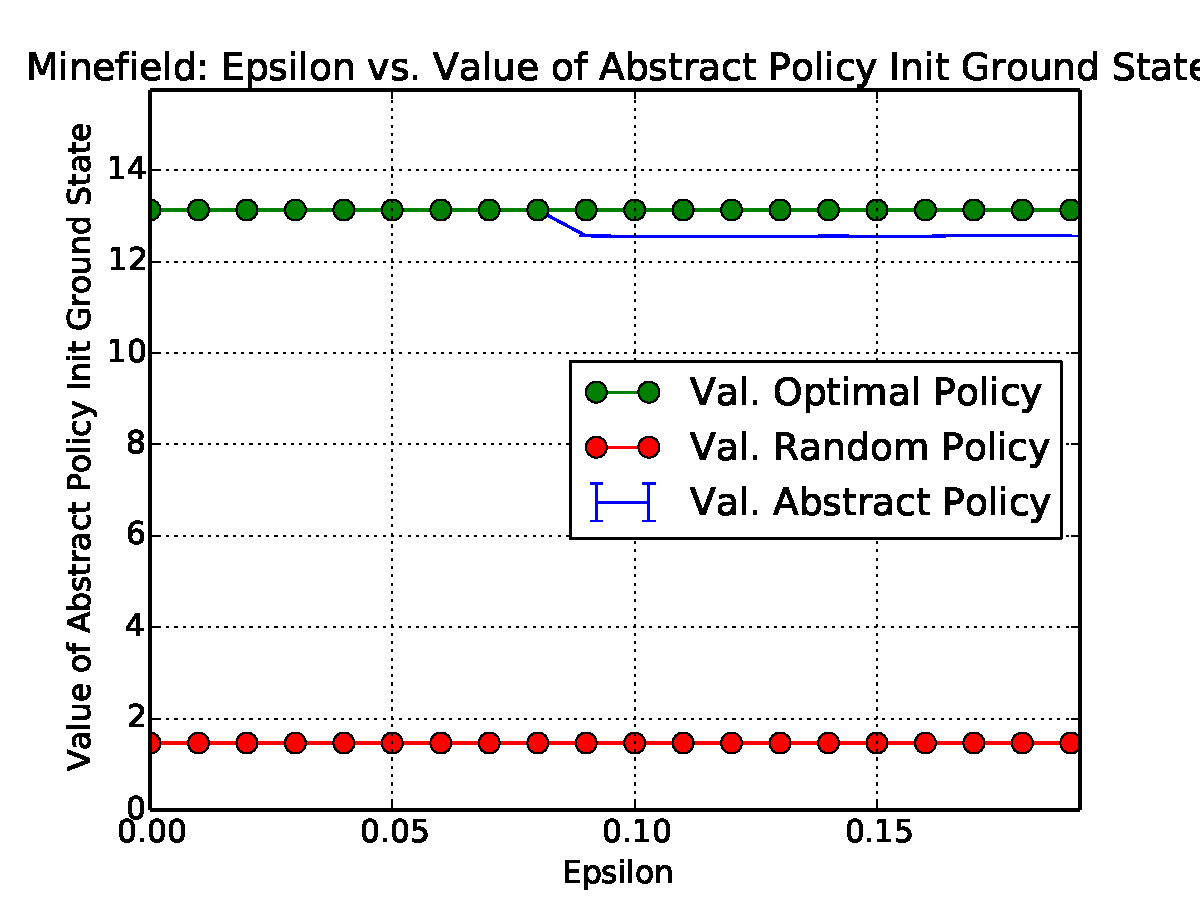
\includegraphics[width=0.48\columnwidth]{figures/minefield_epsilon_vs_value_of_abstract_policy_init_ground_state}}
\subfigure[Random]{
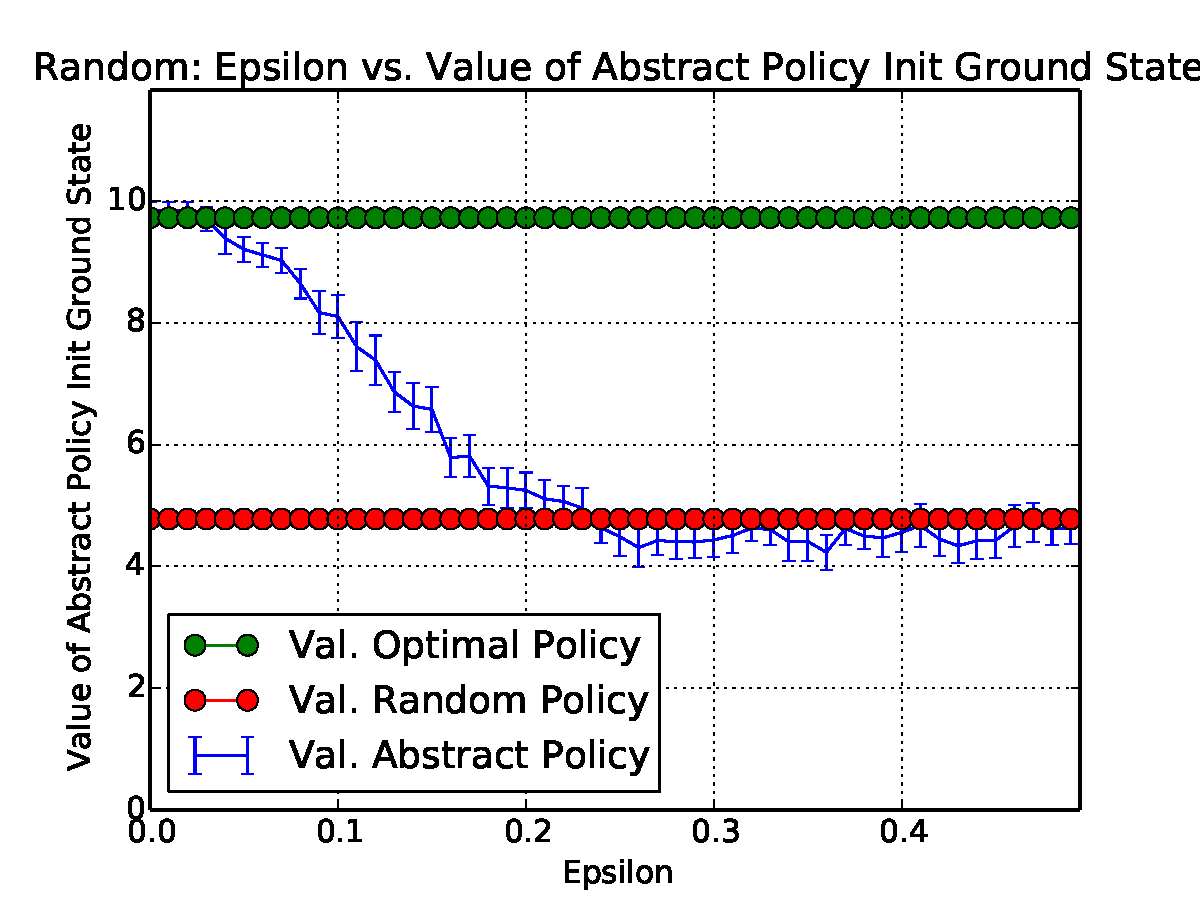
\includegraphics[width=0.48\columnwidth]{figures/random_epsilon_vs_value_of_abstract_policy_init_ground_state}}
\label{fig:eps-states}
\caption{$\epsilon$ vs. the Value under the Abstract Policy in the Initial Ground State}
\end{figure} 
